\section*{سوال ۱}

مفهوم
\lr{AMI}
یا
\lr{Ambient Intelligence}
چیست و آینده آن به چه صورتی است؟

\section*{جواب سوال ۱}

\begin{figure}[H]
	\centering
	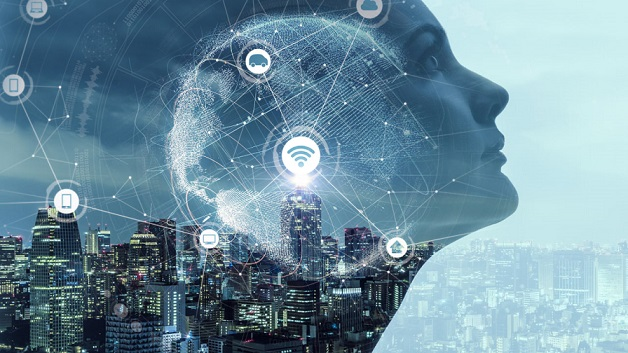
\includegraphics{pic1.jpg}
	\label{fig:label4}
\end{figure}

\lr{Ambient Intelligence (AMI)}
به فناوری و محیطی اشاره دارد که در آن ابزارهای الکترونیکی، سنسورها، دستگاه‌های اکتواتور (موتورهای کوچک برای حرکت یا کنترل محیط) و فناوری‌های پیشرفته دیگر، به طور پیوسته، در هم تنیده و متصل هستند تا یک محیط زنده و هوشمند ایجاد کنند. در این محیط، تکنولوژی به گونه‌ای با زندگی روزمره ادغام شده است که کاربران به صورت تقریباً نامحسوس از آن بهره‌مند می‌شوند. این امکان را به افراد می‌دهد تا بدون نیاز به فهم پیچیدگی‌های فنی، با دستگاه‌های اطراف خود به طور طبیعی تعامل داشته باشند.

\section*{پیشینه AMI}
مفهوم
\lr{AMI}
در دهه 1990 توسعه یافت، زمانی که موسسات تحقیقاتی مانند
\lr{Philips}
و
\lr{MIT Media Lab}
شروع به کاوش در فناوری‌هایی کردند که می‌توانستند به صورت پیوسته و بدون دخالت آشکار کاربر، در زندگی روزمره او تأثیر بگذارند. با پیشرفت‌های سریع در فناوری‌های ارتباطی و شبکه‌ای، ایده‌هایی مانند خانه‌های هوشمند و شهرهای هوشمند به تدریج به واقعیت نزدیک شدند.

\begin{figure}[H]
	\centering
	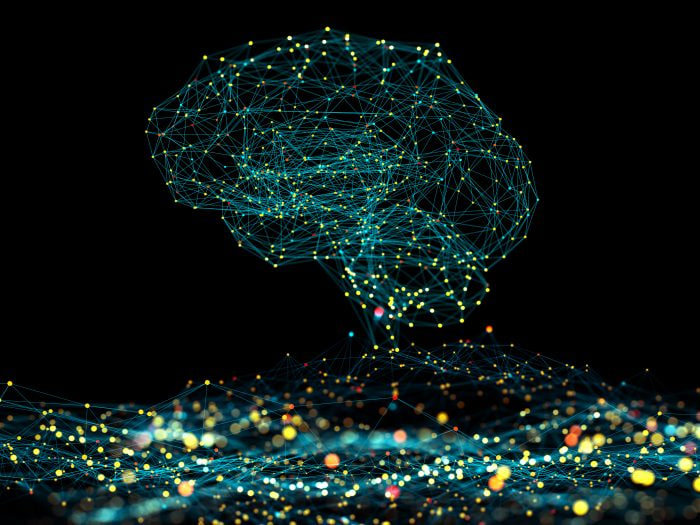
\includegraphics{pic2.jpg}
	\label{fig:label4}
\end{figure}

\section*{حال حاضر و آینده AMI}
در حال حاضر،
\lr{AMI}
در حال پیدا کردن جایگاهی است در بسیاری از جنبه‌های زندگی مدرن، از خانه‌های هوشمند گرفته تا محیط‌های کاری و حتی شهرهای هوشمند. با گسترش اینترنت اشیاء 
\lr{(IoT)}
و فناوری‌های مانند هوش مصنوعی و یادگیری ماشین، این سیستم‌ها به طور فزاینده‌ای می‌توانند اقدامات و نیازهای انسانی را پیش‌بینی کنند و به آنها پاسخ دهند.

آینده‌ی
\lr{AMI}
می‌تواند شامل پیشرفت‌های چشمگیری باشد، از جمله:
\begin{itemize}
	\item انطباق‌پذیری بیشتر: محیط‌ها به طور فعال با نیازها و ترجیحات افراد سازگار خواهند شد.
	\item پیشرفت‌های در حوزه حریم خصوصی و امنیت: با افزایش نگرانی‌های مربوط به داده‌های شخصی، فناوری‌های جدید باید به گونه‌ای طراحی شوند که حفظ حریم خصوصی را تضمین کنند.
	\item همگرایی بیشتر با پوشیدنی‌ها: دستگاه‌های پوشیدنی همچنان با محیط اطراف ادغام خواهند شد، اجازه دادن به کاربران برای انجام تعاملات پیچیده تر با محیط.
	\item استقلال و خودمختاری: سیستم‌های \lr{AMI} ممکن است قادر به انجام تصمیم‌گیری‌های پیچیده‌تر بدون نیاز به دخالت انسانی باشند.
	\item تعاملات انسان-ماشین طبیعی‌تر: با پیشرفت در زمینه شناسایی گفتار و پردازش زبان طبیعی، تعامل با سیستم‌های \lr{AMI} بیش از پیش طبیعی و انسانی خواهد شد.
\end{itemize}
این فناوری‌ها نه تنها زندگی روزمره را آسان‌تر می‌کنند، بلکه می‌توانند برای کمک به افراد معلول، سالمندان و دیگر گروه‌های آسیب‌پذیر در جامعه به کار روند.

\section*{کاربردهای عملی \lr{AMI}}
در دنیای مدرن،
\lr{Ambient Intelligence (AMI)}
به طور فزاینده‌ای در بخش‌های مختلف صنعتی و زندگی روزمره مردم نقش دارد. در حوزه بهداشت و درمان، سیستم‌های 
\lr{AMI}
می‌توانند به نظارت مستمر بر شرایط بیماران کمک کرده و در صورت نیاز به اقدامات اورژانسی، به صورت خودکار به پزشکان هشدار دهند. در زمینه حمل و نقل، استفاده از
\lr{AMI}
به خودروها اجازه می‌دهد تا ترافیک را به طور هوشمندانه تحلیل کرده و مسیرهای بهینه را ارائه دهند. در خرده‌فروشی، فناوری‌های
\lr{AMI}
می‌توانند تجربه خرید را با شناسایی نیازها و عادت‌های خرید مشتریان شخصی‌سازی کنند. در نهایت، در زمینه مدیریت انرژی،
\lr{AMI}
به بهینه‌سازی مصرف انرژی در خانه‌ها و ساختمان‌های تجاری کمک می‌کند، که می‌تواند به کاهش هزینه‌ها و اثرات زیست‌محیطی منجر شود.

\section*{تأثیر \lr{AMI} بر تجربه کاربر}
تأثیر \lr{AMI} بر تجربه کاربر از طریق قابلیت‌های شناسایی الگوهای رفتاری و شخصی‌سازی تجربه‌ها مشخص می‌شود. سیستم‌های هوشمند می‌توانند تنظیمات دستگاه‌های الکترونیکی را بر اساس ترجیحات کاربر تغییر دهند، مانند تنظیم دمای محیط یا روشنایی منزل. این شخصی‌سازی نه تنها راحتی فراهم می‌کند بلکه می‌تواند به بهره‌وری و کاهش مصرف انرژی نیز کمک کند.

\section*{مسائل اخلاقی و حریم خصوصی}
در حالی که \lr{AMI} مزایای زیادی دارد، نگرانی‌های قابل توجهی در مورد حریم خصوصی و مسائل اخلاقی وجود دارد. جمع‌آوری داده‌های شخصی بدون رضایت کامل و آگاهی کاربران می‌تواند خطراتی برای حریم خصوصی ایجاد کند. علاوه بر این، سوءاستفاده از این داده‌ها توسط شرکت‌ها یا هکرها می‌تواند منجر به تهدیدهای امنیتی شود. لذا، طراحی سیستم‌های \lr{AMI} باید با در نظر گرفتن استانداردهای اخلاقی و حفاظت از داده‌های شخصی انجام شود.

\section*{تأثیر اجتماعی و فرهنگی}
تأثیر فرهنگی و اجتماعی \lr{AMI} باید با دقت ارزیابی شود. این فناوری‌ها می‌توانند بر شیوه زندگی، تعاملات اجتماعی و حتی ساختارهای اقتصادی تأثیر بگذارند. تغییر در شغل‌ها و مهارت‌های مورد نیاز برای بازار کار نیز از دیگر تأثیرات است که باید در نظر گرفته شود. این فناوری‌ها می‌توانند به ایجاد جوامع پایدارتر کمک کنند، اما همچنین ممکن است باعث شوند برخی از گروه‌های اجتماعی احساس کنار گذاشته شدن کنند.

مفهوم \textbf{Ambient Intelligence (AMI)} با سیستم‌های نهفته (\textbf{Embedded Systems}) در ارتباط تنگاتنگی قرار دارد. سیستم‌های نهفته رایانه‌های تخصصی هستند که در دستگاه‌های الکترونیکی برای انجام وظایف خاص طراحی شده‌اند. این سیستم‌ها اغلب در برنامه‌هایی که نیاز به پردازش داده‌های محلی، پاسخ‌گویی سریع و ادغام با دنیای فیزیکی دارند، به کار برده می‌شوند. در AMI، سیستم‌های نهفته نقش محوری دارند چرا که به این سیستم‌ها اجازه می‌دهند تا به صورت همه‌جانبه، در محیط‌های فیزیکی ادغام شوند و تجربه‌های کاربری غنی و هوشمندانه‌ای ارائه دهند.

\section*{سیستم‌های نهفته در \lr{AMI}}

\subsection*{تعامل با محیط}
سیستم‌های نهفته در \lr{AMI} می‌توانند از طریق سنسورها و اکچویتورها با محیط اطراف خود تعامل داشته باشند. سنسورها داده‌هایی از محیط جمع‌آوری می‌کنند، مانند دما، رطوبت، نور، حرکت، و صدا. سپس این داده‌ها توسط پردازنده‌های سیستم‌های نهفته تحلیل و پردازش می‌شوند تا اطلاعاتی مفید برای اتخاذ تصمیم‌های هوشمندانه فراهم آورند.

\subsection*{خودکارسازی و پاسخگویی}
سیستم‌های نهفته می‌توانند فعالیت‌های خودکاری مانند کنترل دما، روشنایی، و سیستم‌های امنیتی را اجرا کنند. به عنوان مثال، در یک خانه هوشمند، سیستم‌های نهفته ممکن است تشخیص دهند که هیچ کس در اتاق حضور ندارد و به صورت خودکار چراغ‌ها را خاموش کنند تا انرژی صرفه‌جویی شود.

\subsection*{هوش مصنوعی و یادگیری ماشین}
برای رسیدن به سطح بالایی از هوشمندی، سیستم‌های نهفته در \lr{AMI} اغلب با الگوریتم‌های یادگیری ماشین و هوش مصنوعی تجهیز می‌شوند. این الگوریتم‌ها به سیستم‌ها امکان می‌دهند تا از تجربیات گذشته یاد بگیرند، الگوهای رفتاری را شناسایی کنند، و پیش‌بینی‌هایی در مورد نیازهای آینده کاربران داشته باشند.

\subsection*{امنیت و حریم خصوصی}
یکی از چالش‌های اصلی سیستم‌های نهفته در \lr{AMI} حفاظت از اطلاعات شخصی و حفظ حریم خصوصی کاربران است. با توجه به میزان داده‌های حساسی که جمع‌آوری و پردازش می‌شود، لازم است سیستم‌های امنیتی و رمزنگاری پیشرفته‌ای برای محافظت از این اطلاعات در برابر دسترسی‌های غیرمجاز ادغام شوند.

\subsection*{بهینه‌سازی مصرف انرژی}
سیستم‌های نهفته باید بتوانند با مصرف کم انرژی کار کنند تا به توسعه پایدار کمک کنند. در \lr{AMI}، این مسئله به معنای طراحی سخت‌افزار و نرم‌افزارهایی است که کارآمدی انرژی را به حداکثر برسانند و در عین حال کارایی بالایی داشته باشند.

در نهایت، سیستم‌های نهفته به عنوان مغز و مرکز کنترل در مفهوم \textbf{\lr{Ambient Intelligence}} عمل می‌کنند، که به آن‌ها اجازه می‌دهد تا به صورت همزمان هم هوشمند و هم پنهان باقی بمانند. این امر موجب می‌شود تا تجربه‌های کاربری به شکلی طبیعی و بی‌درز با زندگی روزمره ادغام شوند.
